\section{Current Evidence, Execution, and Verification}\label{ec:execution56}
The R57 execution is a new repository-published run of the disclosed recovered design. It contains 186 primary timed method runs, 39 exact-target and encoding extension runs, and nine separate deterministic mechanical replays. Primary and extension cases, method targets, seeds, allowances and outputs remain individually identifiable. Source hashes are recorded before the timed calls and checked after them. The executed design was inspected during earlier development and is not described as an unseen confirmatory sample.

\subsection{Publication recovery and execution provenance}
The R56 review correctly found no revised scientific manuscript in its Git tree. A complete local R56 package was subsequently recovered and its 225 corrected records and 200 certificate byte hashes were audited against the saved manifest. That local package was development input to R57; it is not evidence that the earlier branch was complete. Its original hash is retained in the R57 protocol. The current article's numerical statements instead derive from the new, source-frozen R57 repository execution.

The recovered executor already preserves a completed enumeration incumbent under an outer alarm through caller-owned progress, and records the completed-book count. It also encodes enormous rejected state requests by hexadecimal size and bit length. R57 uses these corrections from the beginning. No completed old result is silently overwritten: earlier published R54 records stay unchanged, and the recovered local R56 archive remains separately identified. The different missing 269-run R55 local development archive is neither invented from a protocol nor counted among current records. Its three historical governance files remain on their original branch.

\subsection{Clocks and outcome definitions}
Every timed method uses a fresh process, single-thread numerical libraries and a two-GiB address-space limit. The optimization allowance is one half-second or two seconds; process setup is measured separately. Screening includes seed search, forced bounds and reduced solving within the same total algorithm allowance as its direct comparator. Optimization, proof serialization and independent checking have separate measured costs. A parent cutoff and a Python signal alarm are different safeguards; native-process overruns and the last completed phase remain observable.

An unchanged certificate initially receives twelve seconds of checking. Initial timeouts may receive a separately recorded ninety-second check, with the original status and bytes preserved. A valid fallback interval need not meet the requested tolerance. Exact completion means zero rational width; numerical MIP cost-envelope results have a separate status; an oversized-state rejection does not supply an optimum. The raw record preserves solver residuals and envelope error rather than treating tiny numerical bracket reversals as negative certified gaps.

\subsection{Independent recurrences and proof economics}
The price checker uses a backward at-most-budget recurrence, independently validates original lotteries and verifies the complete leaf cover. The deficit checker rebuilds kernels and tests Bellman inequalities by direct predecessor enumeration, together with an attaining path, the rounding bound and an original-policy lower certificate. Neither checker imports its optimizer. Shared parsing of exact rationals and separately validated original-policy feasibility do not share the optimization recurrence.

The direct deficit checker has conservative arithmetic cost $O(k^2N^2Q+mN^2Q^2)$, which can exceed the optimizer's fast-convolution cost. Both are measured. Raw and gzip proof sizes include the model, policy and full proof; deterministic gzip timestamps do not certify mathematical correctness. Numerator and denominator bit lengths are recorded separately. Hexadecimal serialization avoids a decimal conversion limit but does not remove large-integer arithmetic. Tests include a full certificate exceeding twenty thousand bits, a pre-allocation rejected enormous grid, and seven altered-certificate classes.

\path{SEARCH_MECHANICS.csv} records evaluated and created nodes, completed oracle calls, root and final gaps, live leaves, depth, required-set sizes, incumbent updates, pruning categories and final book cardinality. Root gap contraction is relative to the initialized gross bound. Direct-tree standalone forced fixings are not conflated with separate screening exclusions. Nine deterministic replays expose every tested price and required/forbidden set and compare fixed-book selection with lexicographic enumeration at equal book count, not equal arithmetic work. Figure~\ref{fig:trajectory56} retains every recorded epoch for two specified eight-history exact-target cases.
\begin{figure}[htbp]\centering
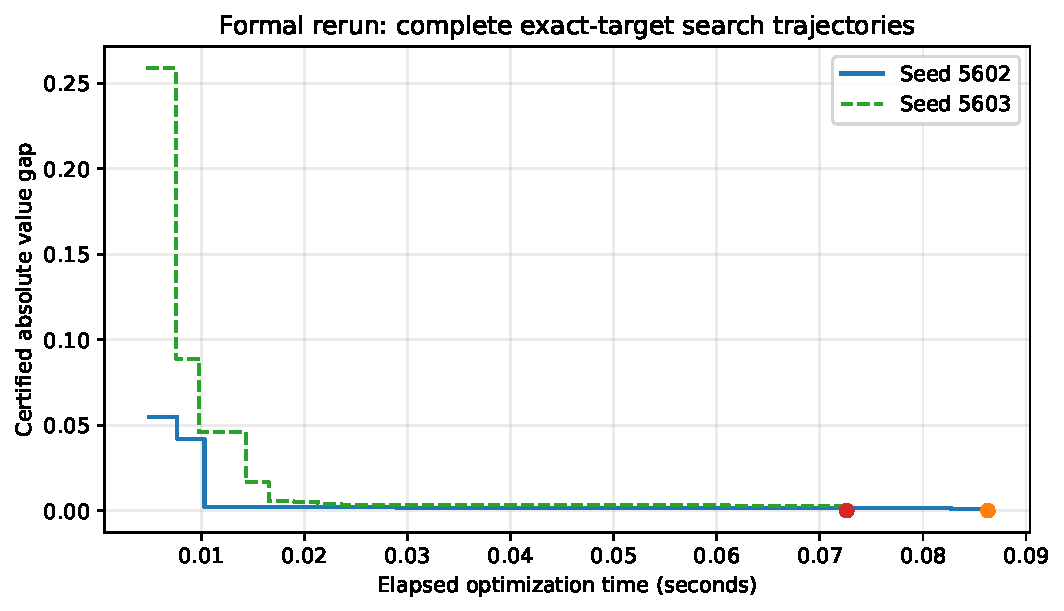
\includegraphics[width=\textwidth]{revisions/or-r58-structural-referee-20260926/generated/exact_trajectories.pdf}
\caption{Complete recorded exact-target price trajectories for the two eight-history instances requiring branching. Every recorded epoch is retained. The final circles denote zero rational width; elapsed times are those of the published two-second-limit runs, not the later mechanical replay.}\label{fig:trajectory56}
\end{figure}


\subsection{Complete reader and preservation checks}
R57 starts from the last genuinely published R54 scientific commit, not from a reviewer-output commit. Exact root predecessors are retained. A complete Git-blob manifest checks all inherited files; the current reader's TeX recorder checks the sources actually assembled. Main, companion, response, generated figures and tables, code/data package and source/result hashes identify one stable review object. Successful publication and build checks do not establish editorial acceptance.
